
%----------------------------------------------------------------------------------------
%	PACKAGES AND OTHER DOCUMENT CONFIGURATIONS
%----------------------------------------------------------------------------------------

\documentclass[paper=a4, fontsize=11pt]{article} % A4 paper and 11pt font size

\usepackage[T1]{fontenc} % Use 8-bit encoding that has 256 glyphs
\usepackage{fourier} % Use the Adobe Utopia font for the document - comment this line to return to the LaTeX default
\usepackage[english]{babel} % English language/hyphenation
\usepackage{amsmath,amsfonts,amsthm} % Math packages

\usepackage{sectsty} % Allows customizing section commands
\allsectionsfont{\raggedright \normalfont\scshape} % Make all sections centered, the default font and small caps

\usepackage{fancyhdr} % Custom headers and footers
\pagestyle{fancyplain} % Makes all pages in the document conform to the custom headers and footers
\fancyhead{} % No page header - if you want one, create it in the same way as the footers below
\fancyfoot[L]{} % Empty left footer
\fancyfoot[C]{} % Empty center footer
\fancyfoot[R]{\thepage} % Page numbering for right footer
\renewcommand{\headrulewidth}{0pt} % Remove header underlines
\renewcommand{\footrulewidth}{0pt} % Remove footer underlines
\setlength{\headheight}{13.6pt} % Customize the height of the header

\usepackage{parskip}
\setlength{\parindent}{15pt}
 \usepackage{graphicx}
 \usepackage{epstopdf}
\usepackage{caption}
\usepackage{subcaption}
%\numberwithin{equation}{section} % Number equations within sections (i.e. 1.1, 1.2, 2.1, 2.2 instead of 1, 2, 3, 4)
%\numberwithin{figure}{section} % Number figures within sections (i.e. 1.1, 1.2, 2.1, 2.2 instead of 1, 2, 3, 4)
%\numberwithin{table}{section} % Number tables within sections (i.e. 1.1, 1.2, 2.1, 2.2 instead of 1, 2, 3, 4)

\setlength\parindent{0pt} % Removes all indentation from paragraphs - comment this line for an assignment with lots of text

%----------------------------------------------------------------------------------------
%	TITLE SECTION
%----------------------------------------------------------------------------------------

\newcommand{\horrule}[1]{\rule{\linewidth}{#1}} % Create horizontal rule command with 1 argument of height

\title{	
\normalfont \normalsize 
\textsc{Nuclear Engineering, UC Berkeley} \\ [25pt] % Your university, school and/or department name(s)
\horrule{0.5pt} \\[0.4cm] % Thin top horizontal rule
\huge ME 280A Finite Element Analysis \\HOMEWORK 3: Potential and efficient solution techniques  \\  % The assignment title
\horrule{2pt} \\[0.5cm] % Thick bottom horizontal rule
}

\author{Xin Wang} % Your name

\date{\normalsize\today} % Today's date or a custom date

\begin{document}

\maketitle % Print the title

\newpage
\section{Introduction}
The objective of this project is to solve a 1-D differential equation using linear elements.  

\begin{eqnarray}
\frac{d}{dx}(A_1(x) \frac{du}{dx}) &=& f(x)\nonumber\\
f(x)&=&256sin(\frac{3\pi kx}{4})cos(16 \pi x) \nonumber\\
A_1(x)& = & piecewise\nonumber\\
L&=&1 \nonumber\\
u(0)& =& 0 \nonumber\\
A1(L)\frac{du}{dx}(L) &=& 1 \nonumber\\
\end{eqnarray}

$A_1$ is a piece wise function, defined as bellow:

\begin{eqnarray}
For & 0.0 \leq x < 0.1 :& A_1 = 2.0 \nonumber\\
For & 0.1 \leq x < 0.2 :& A_1 = 2.5 \nonumber\\
For & 0.2 \leq x < 0.3 :& A_1 = 1.25 \nonumber\\
For & 0.3 \leq x < 0.4 :& A_1 = 0.25 \nonumber\\
For & 0.4 \leq x < 0.5 :& A_1 = 4.0 \nonumber\\
For & 0.5 \leq x < 0.6 :& A_1 = 1.75 \nonumber\\
For & 0.6 \leq x < 0.7 :& A_1 = 0.5 \nonumber\\
For & 0.7 \leq x < 0.8 :& A_1 = 0.75 \nonumber\\
For & 0.8 \leq x < 0.9 :& A_1 = 3.25\nonumber\\
For & 0.9 \leq x \leq 1.0 :& A_1 = 1.0
\end{eqnarray}

%%%%%%%%%%%%%%%%%%%%%%%%%%%%%%%%%%%%%%%%%%%%%%%%%%%%%%%%%%%%%%%%%%%%%%%%%%%%%%%%%%%%%%%%%%%%%%%%%%%%%%%%%%%%%%%%%%%%%%%%%%%%%%%%%%%
%analytical solution
%%%%%%%%%%%%%%%%%%%%%%%%%%%%%%%%%%%%%%%%%%%%%%%%%%%%%%%%%%%%%%%%%%%%%%%%%%%%%%%%%%%%%%%%%%%%%%%%%%%%%%%%%%%%%%%%%%%%%%%%%%%%%%%%%%%
\section{Analytical solution}

The general solution for this equation on every segment can be found after two integrations:
\begin{eqnarray}
\label{du_ana}
A_1(x)\frac{du}{dx}&=& \int 256sin(\frac{3\pi kx}{4})cos(16 \pi x) dx\nonumber\\
&=& \int 128[sin(\frac{67 \pi x}{4}) - sin(\frac{61 \pi x}{4})]\nonumber\\
&=& \frac{512(67cos(\frac{61\pi x}{4})- 61cos(\frac{67\pi x}{4}))}{4087\pi} + C1
\end{eqnarray}

\begin{eqnarray}
\frac{du}{dx} &=& \frac{1}{A_1(x)} (\frac{ 512( 67cos( \frac{61\pi x}{4} )- 61cos( \frac{67\pi x}{4} ) ) }  {4087\pi} + C1)
\end{eqnarray}

Integrating $\frac{du}{dx}$ and applying the boundary condition at x=0, we obtain the analytical solution for the differencial equation:

\begin{eqnarray}
u(x)&=& \frac{\frac{137216sin(\frac{61\pi x}{4})}{61\pi}- \frac{124928sin(\frac{67\pi x}{4}))}{67\pi}}{4087\pi} + \frac{C1x} {A_1(x)} + C2
\end{eqnarray}



At the interface of each segments$x_N$(N=1,...,10), the function u and its derivation is continuous, i.e.,

\begin{eqnarray}
u(x_N^+) = u(x_N^-) \nonumber\\
A1(x_N^+)\frac{du} {dx}(x_N^+) = A1(x_N^1)\frac{du}{dx}(x_N^-)
\end{eqnarray}

In particular, at the left endpoint, $u(0) = u_0 = 0$ and at the right end point, $A1(L)\frac{du}{dx} (L) = A1(L)(\frac{du}{dx})_N = 1 $ .

Applying these boundary conditions and continuation conditions at the interfaces, we can solve the equation system and obtain the analytical solution:

\begin{eqnarray}
For & 0.0 \leq x < 0.1 :& C_1 = 1.1692 \nonumber\\
For & 0.1 \leq x < 0.2 :& C_1 = 1.1692 \nonumber\\
For & 0.2 \leq x < 0.3 :& C_1 = 1.1692 \nonumber\\
For & 0.3 \leq x < 0.4 :& C_1 = 1.1692 \nonumber\\
For & 0.4 \leq x < 0.5 :& C_1 = 1.1692 \nonumber\\
For & 0.5 \leq x < 0.6 :& C_1 = 1.1692 \nonumber\\
For & 0.6 \leq x < 0.7 :& C_1 = 1.1692 \nonumber\\
For & 0.7 \leq x < 0.8 :& C_1 = 1.1692 \nonumber\\
For & 0.8 \leq x < 0.9 :& C_1 = 1.1692\nonumber\\
For & 0.9 \leq x \leq 1.0 :& C_1 = 1.1692
\end{eqnarray}


\begin{eqnarray}
For & 0.0 \leq x < 0.1 :& C_2 = 0 \nonumber\\
For & 0.1 \leq x < 0.2 :& C_2 = 0.0101\nonumber\\
For & 0.2 \leq x < 0.3 :& C_2 = -0.0964 \nonumber\\
For & 0.3 \leq x < 0.4 :& C_2 = =1.4040 \nonumber\\
For & 0.4 \leq x < 0.5 :& C_2 = 0.2742 \nonumber\\
For & 0.5 \leq x < 0.6 :& C_2 = 0.1166 \nonumber\\
For & 0.6 \leq x < 0.7 :& C_2 = -0.8391 \nonumber\\
For & 0.7 \leq x < 0.8 :& C_2 = -0.2384 \nonumber\\
For & 0.8 \leq x < 0.9 :& C_2 = 0.7997\nonumber\\
For & 0.9 \leq x \leq 1.0 :& C_2 = 0.0931
\end{eqnarray}
%%%%%%%%%%%%%%%%%%%%%%%%%%%%%%%%%%%%%%%%%%%%%%%%%%%%%%%%%%%%%%%%%%%%%%%%%%%%%%%%%%%%%%%%%%%%%%%%%%%%%%%%%%%%%%%%%%%
%section Finite Element Method
%%%%%%%%%%%%%%%%%%%%%%%%%%%%%%%%%%%%%%%%%%%%%%%%%%%%%%%%%%%%%%%%%%%%%%%%%%%%%%%%%%%%%%%%%%%%%%%%%%%%%%%%%%%%%%%%%%%

\section{Finite Element Method}
The first step of FEM is to derive the weak form of the differential equation:

Find u, u|$\Gamma u$ =d, such that $\forall v$, v|$\Gamma u$ =0

\begin{eqnarray}
\int_{\Omega} \frac{dv}{dx} A_1 \frac{du}{dx} dx = \int_{\Omega} fv dx + tv \mid _{\Gamma t}
\end{eqnarray}


We approximate the real solution u by

\begin{eqnarray}
u(x) = \sum_{j=1}^{N} a_j \phi_j(x)
\end{eqnarray}

and we choose the test function v with the same approximation functions

\begin{eqnarray}
v(x) = \sum_{i=1}^{N} b_i \phi_i(x)
\end{eqnarray}

where N is the number of degree of freedom(number of nodes). 


Then the equation becomes:

\begin{eqnarray}
\int_{\Omega} \frac{d}{dx} (\sum_{j=1}^{N+1} a_j \phi_j(x)) A_1 \frac{d}{dx} (\sum_{i=1}^{N+1} b_i \phi_i(x))dx = \int_{\Omega} f (\sum_{i=1}^{N+1} b_i \phi_i(x)) dx + (\sum_{i=1}^{N+1} b_i \phi_i(x) t) \mid _{\Gamma t}, \forall b_i
\end{eqnarray}


We can regroup the terms into:

\begin{eqnarray}
\sum_{i=1}^{N+1} b_i \int_{\Omega} (\sum_{j=1}^{N+1} a_j \frac{d}{dx} \phi_j(x) A_1 \frac{d}{dx} \phi_i(x)) dx = \sum_{i=1}^{N+1} b_i \int_{\Omega} f \phi_i(x) dx + \sum_{i=1}^{N+1} b_i (\phi_i(x) t) \mid _{\Gamma t}
\end{eqnarray}

As the equation should be valid for any $b_i$, we obtain the matrix system to solve:
 
\begin{eqnarray}
K_{ij} &=& \int_{\Omega} \frac{d}{dx} \phi_j(x) A_1 \frac{d}{dx} \phi_i(x) dx \nonumber\\
R_i &=& \int_{\Omega} f \phi_i(x) dx + \phi_i(x) t \mid _{\Gamma t}\nonumber\\
K a &=& R
\end{eqnarray}


In this homework, piece-wise linear, quadratic or cubic basis functions are used. The numerical computation is carried over the corresponding master elements and mapped to the global elements. 

Shape functions are defined for elements with different polynomial orders(figure \ref{fig:shape}).

Linear shape functions are:
\begin{eqnarray}
\hat{\phi_1} &=& \frac{1-\xi}{2}\nonumber\\
\hat{\phi_2} &=& \frac{1+\xi}{2}
\end{eqnarray}

and

\begin{eqnarray}
\frac{d\hat{\phi_1}}{d\xi} &=& -\frac{1}{2}\nonumber\\
\frac{d\hat{\phi_2}}{d\xi} &=& \frac{1}{2}
\end{eqnarray}

Corresponding global coordinate x can be calculate x from $\xi$:

\begin{equation}
x = \sum{\chi _i \hat{\phi _i}}
\end{equation} 
where $\chi_i$ are the coordinates of the nodes in the global element. 

The method to compute the matrices K and R element by element and assembling procedures are the same as in homework 1. The difference for higher order elements is the size of Ke and Re.   

The data structure used for store the matrix K is a 3xN matrix where only three numbers in the 2x2 element K matrix are stores.

\begin{eqnarray}
ke\_table = \{ k_{11}^1, k_{12}^1, k_{22}^1 \\
               k_{11}^2, k_{12}^2, k_{22}^2 \} 
\end{eqnarray}
 
 \subsection{Boundary condition}

As discussed in the previous homeworks, for Dirichlet BC on u(0):

Apllying K(1,1) =1 and K(1, 2) =0 

R(1) = u(0)

For Dirichlet BC on u(L):

K(N,N) =1 and K(N, 1:N-1) =0 

R(N) = u(L)

After the modification, a = K/R results in for the line corresponds to Dirichlet boundary condition: 

a(1) = R(1)/K[1,1] = R(1)

or
 
a(N) = R(N)/K[N,N] = R(N) 

\subsubsection{Neumann boundary condition}
Neumann boundary condition gives the value of traction $A1(x)\frac{du}{dx}$ on an end point.

For Neumann BC on x=0:

 $R(1) = R(1) + A_1 \frac{du}{dx}[x=0] $


For Neumann BC on x=L:

 $R(N)=R(N)+ A_1 \frac{du}{dx}[x=L] $
%%%%%%%%%%%%%%%%%%%%%%%%%%%%%%%%%%%%%%%%%%%%%%%%%%%%%%%%%%%%%%%%%%%%%%%%%%%%%%%%%%%%%%%%%%%%%%%%%%%%%%%%%%%%%%%%%%%%%%%%%%%%%%%%%%%
%Section: preconditioned conjugate-gradiant solver
%%%%%%%%%%%%%%%%%%%%%%%%%%%%%%%%%%%%%%%%%%%%%%%%%%%%%%%%%%%%%%%%%%%%%%%%%%%%%%%%%%%%%%%%%%%%%%%%%%%%%%%%%%%%%%%%%%%%%%%%%%%%%%%%%%%
\section{Preconditioned conjugate-gradient solver}
There are two approaches to solve the equation for [K]{a} = {R}, direct and iterative. The number of operation in direct solvers are  $O(N^3)$. They are employed when the number of unknowns are not very large, and there are multiple load vectors. Iterative solver are prefered when the systems are very large. Conjugate gradient type iterative techniques need $O(N^2)$ operations. 

We define a potential(eq\ref{eq: Pi}) whose derivative is the residual of the equation to solve. So the minimizer of the potential $\Pi$ is the solution to the discrete system. 
\begin{eqnarray}
\bigtriangledown \Pi = [K]\{a\} - \{R\}
\end{eqnarray}

\begin{eqnarray}
\label{eq: Pi}
\Pi = \frac{1}{2} \{a\}^T [K] \{a\} - \{a\}^T\{R\}
\end{eqnarray}

\begin{eqnarray}
\label{eq: residual}
\{r\}^i = - \bigtriangledown \Pi = \{R\} - [K] \{a\}^i \nonumber\\
\{a\}^{i+1} = \{a\}^i + \lambda^i \{r\}^i
\end{eqnarray}

The idea of steepest descent is to find this minimizer of potential by going to the direction of the gradiant of the potential, i.e. $\{a\} ^{i+1} = \{a\} ^i + \lambda ^i \{z\} ^i $, where $\{z\}^i = \{r\}^i + \theta ^i\{z\}^{i-1}$.

The coefficient $\theta$ is chosen so that {z} is [K] conjugate to $\{z\}^{i-1}$, i.e.,

\begin{eqnarray}
\{z\}^{T, i} [K] \{z\} ^{i-1} =0 \nonumber\\
\theta^i = - \frac{\{r\}^{T,i} [K] \{z\} ^ {i-1}} {\{z\} ^{T,i-1} [K] \{z\}^{i-1} }
\end{eqnarray}

Looking for $\lambda$ to minimize the potential, we force $\frac{\partial {\Pi}}{\partial \lambda ^i} =0 $ and solve for $\lambda$:

\begin{eqnarray}
\lambda ^i = \frac{ \{z\}^{T,i} \{r\}^i} { \{z\}^{T,i}[K]\{z\}^i}
\end{eqnarray}

\subsection{Preconditioning of [K]}
The rate of convergence of the CG method is related to the condition number

\begin{eqnarray}
\| \{a\} - \{ a\}^i \| _K \leq (\frac{ \sqrt{C([K]) -1} }{ \sqrt{C([K]) + 1} }) ^i \| \{a\} - \{a\} ^1 \| _K
\end{eqnarray}

To reduce the condition number, preconditioning of [K] is done by forming the transformation of variables:
\begin{eqnarray}
\{a\} = [T] \{ A\} \nonumber\\
\bar{[K]} = [T] ^T [K] [T] 
\end{eqnarray} 

Diagonal preconditioning is an inexpensive widely used, where [T] is defined from the diaganol of [K] as:
\begin{eqnarray}
T_{ij} = \frac{1} { \sqrt{ K_{ij} } }, i,j = 1, ... ndof 
\end{eqnarray}

\subsection{iteration}
Starting from an initial guess for $\{a\}^0$, we can calculate the residual defined as in equation \ref{eq: residual}.

\begin{eqnarray}
\label{eq: residual}
\{r\}^0 &=& - \bigtriangledown \Pi = \{R\} - [K] \{a\}^0 \nonumber\\
\{z\}^0 &=& \{r\}^0 \nonumber\\
\lambda ^0 &=& \frac{ \{z\}^{T,0} \{r\}^0} { \{z\}^{T,0}[K]\{z\}^0} \nonumber\\
\{a\}^{1} &=& \{a\}^0 + \lambda^0 \{z\}^0
\end{eqnarray}

For iteration i >0, 
\begin{eqnarray}
\{r\}^i &=& \{R\} - [K] \{a\}^i \nonumber\\
\theta^i &=& - \frac{\{r\}^{T,i} [K] \{z\} ^ {i-1}} {\{z\} ^{T,i-1} [K] \{z\}^{i-1} }\nonumber\\
\{z\} &=& \{r\} ^i + \theta ^i \{z\} ^{i-1} \nonumber\\
\lambda ^i &=& \frac{ \{z\}^{T,i} \{r\}^i} { \{z\}^{T,i}[K]\{z\}^i} \nonumber\\
\{a\} ^{i+1} &=& \{a\} ^i + \lambda ^i \{z\} ^i  \nonumber\\
\end{eqnarray}

and compute the error for each iteration as:

\begin{eqnarray}
e^i = \frac{\|\{a\}^i - \{a\}^i \| _K } { \| \{ a\}^i \| _k} = \frac{ \mid \lambda ^i \mid \| \{z\} \| _K }{ \| \{ a\} ^i _K \|} 
\end{eqnarray}

If $e^i < \tau$ stop, otherwise reiterate. 

%%%%%%%%%%%%%%%%%%%%%%%%%%%%%%%%%%%%%%%%%%%%%%%%%%%%%%%%%%%%%%%%%%%%%%%%%%%%%%%%%%%%%%%%%%%
\section{Error Calculations}
The error is defined as 

\begin{eqnarray}
e^N = \frac{\| u -u^N \| _{A_1(\Omega)}} {\| u \| _{A_1 (\Omega)}} \nonumber\\
\| u \| _{A_1 (\Omega)} = \sqrt{\int_{\Omega} \frac{du}{dx} A_1 \frac{du}{dx} dx} = \sqrt{\int_{\Omega} A_1(\frac{du}{dx})^2 dx}\nonumber\\
\| u -u^N \| _{A_1(\Omega)} = \sqrt{\int_{\Omega} A_1 (\frac{d(u-u^N)}{dx})^2 dx}
\end{eqnarray}

To compute the error numerically, we calculate the two following quantities element by element, and then assemble them to obtain the overall error:

\begin{eqnarray}
\| u \| _{A_1 (\Omega)}^2 &=&\int_{\Omega} A_1(\frac{du}{dx})^2 dx\nonumber\\
\| u -u^N \| _{A_1(\Omega)} ^2 &=& \int_{\Omega} A_1 (\frac{d(u-u^N)}{dx})^2 dx\nonumber\\
&=& A_1 \int_{\Omega} (\frac{du}{dx} - \frac{du_N}{dx})^2 dx\nonumber\\
&=& A_1 \sum_{e=1}^{N_e} \int_{x_e}^{x_{e+1}} (\frac{du}{dx} - \frac{du_N}{dx})^2 dx \nonumber\\
&=& A_1 \sum_{e=1}^{N_e} \int_{-1}^{1} (\frac{du}{d\xi} - \frac{du_N}{d\xi})^2 J d\xi
\end{eqnarray}

%%%%%%%%%%%%%%%%%%%%%%%%%%%%%%%%%%%%%%%%%%%%%%%%%%%%%%%%%%%%%%%%%%%%%%%%%%%%%%%%%%%%%%%%%%%%%%%%%%%%%%%%%%%%%%%%%%%
%section postprocessing
%%%%%%%%%%%%%%%%%%%%%%%%%%%%%%%%%%%%%%%%%%%%%%%%%%%%%%%%%%%%%%%%%%%%%%%%%%%%%%%%%%%%%%%%%%%%%%%%%%%%%%%%%%%%%%%%%%%
\section{Postprocessing}
The postprocessing is more complicated for higher order element. In order to plot the result, we calculate the value of the numerical solution for 10 points in each elements. For any given $\xi$, the corresponding value for the solution is calculated, as well as the global coordinate x for the given $\xi$:

\begin{eqnarray}
 u(x) &=& u(x(\xi))=\sum_{i=1}^{P+1} a_i^e \hat{\phi_i}\nonumber\\
 x(\xi) &=& \sum x^e \hat{\phi}(\xi)
 \end{eqnarray} 

For each element, we can also calculate the derivative of u(x):

\begin{eqnarray}
\frac{du}{dx} = \frac{d}{dx} \sum_{i=1}^{P+1} a_i \phi_i = (\frac{d}{d\xi}\sum_{i=1}^{P+1} a_i \hat{\phi_i})\frac{d\xi}{dx}
\end{eqnarray}

%%%%%%%%%%%%%%%%%%%%%%%%%%%%%%%%%%%%%%%%%%%%%%%%%%%%%%%%%%%%%%%%%%%%%%%%%%%%%%%%%%%%%%%%%%%%%%%%%%%%%%%%%%%%%%%%%%%%%%%%%%%%%%%%%%%
%section results
%%%%%%%%%%%%%%%%%%%%%%%%%%%%%%%%%%%%%%%%%%%%%%%%%%%%%%%%%%%%%%%%%%%%%%%%%%%%%%%%%%%%%%%%%%%%%%%%%%%%%%%%%%%%%%%%%%%%%%%%%%%%%%%%%%%

\section{Results}

Minimum number of elements and number of nodes to achieve to error criteria for different order of elements are tabulated bellow. $N_{Opt}$ drops dramatically with the order of the elements. 
\begin{table}
\begin{center}
  \begin{tabular}{ l | c | c}
    \hline
    P & $Ne_{opt}$ & $N_{opt} = Ne_{Opt} * P + 1 $\\ \hline
    1 & 1348 & 1349\\ \hline
    2 &  94 & 189\\ \hline
    3 & 34 & 103\\ \hline
    \hline
  \end{tabular}
  \caption{Minimum number of nodes needed for the error criteria}
\end{center}
\end{table}

The numerical solution and the analytical solution are compared in figure \ref{fig:solution}. 


% \begin{figure}
%         \centering
%         \begin{subfigure}[b]{\textwidth}
%                 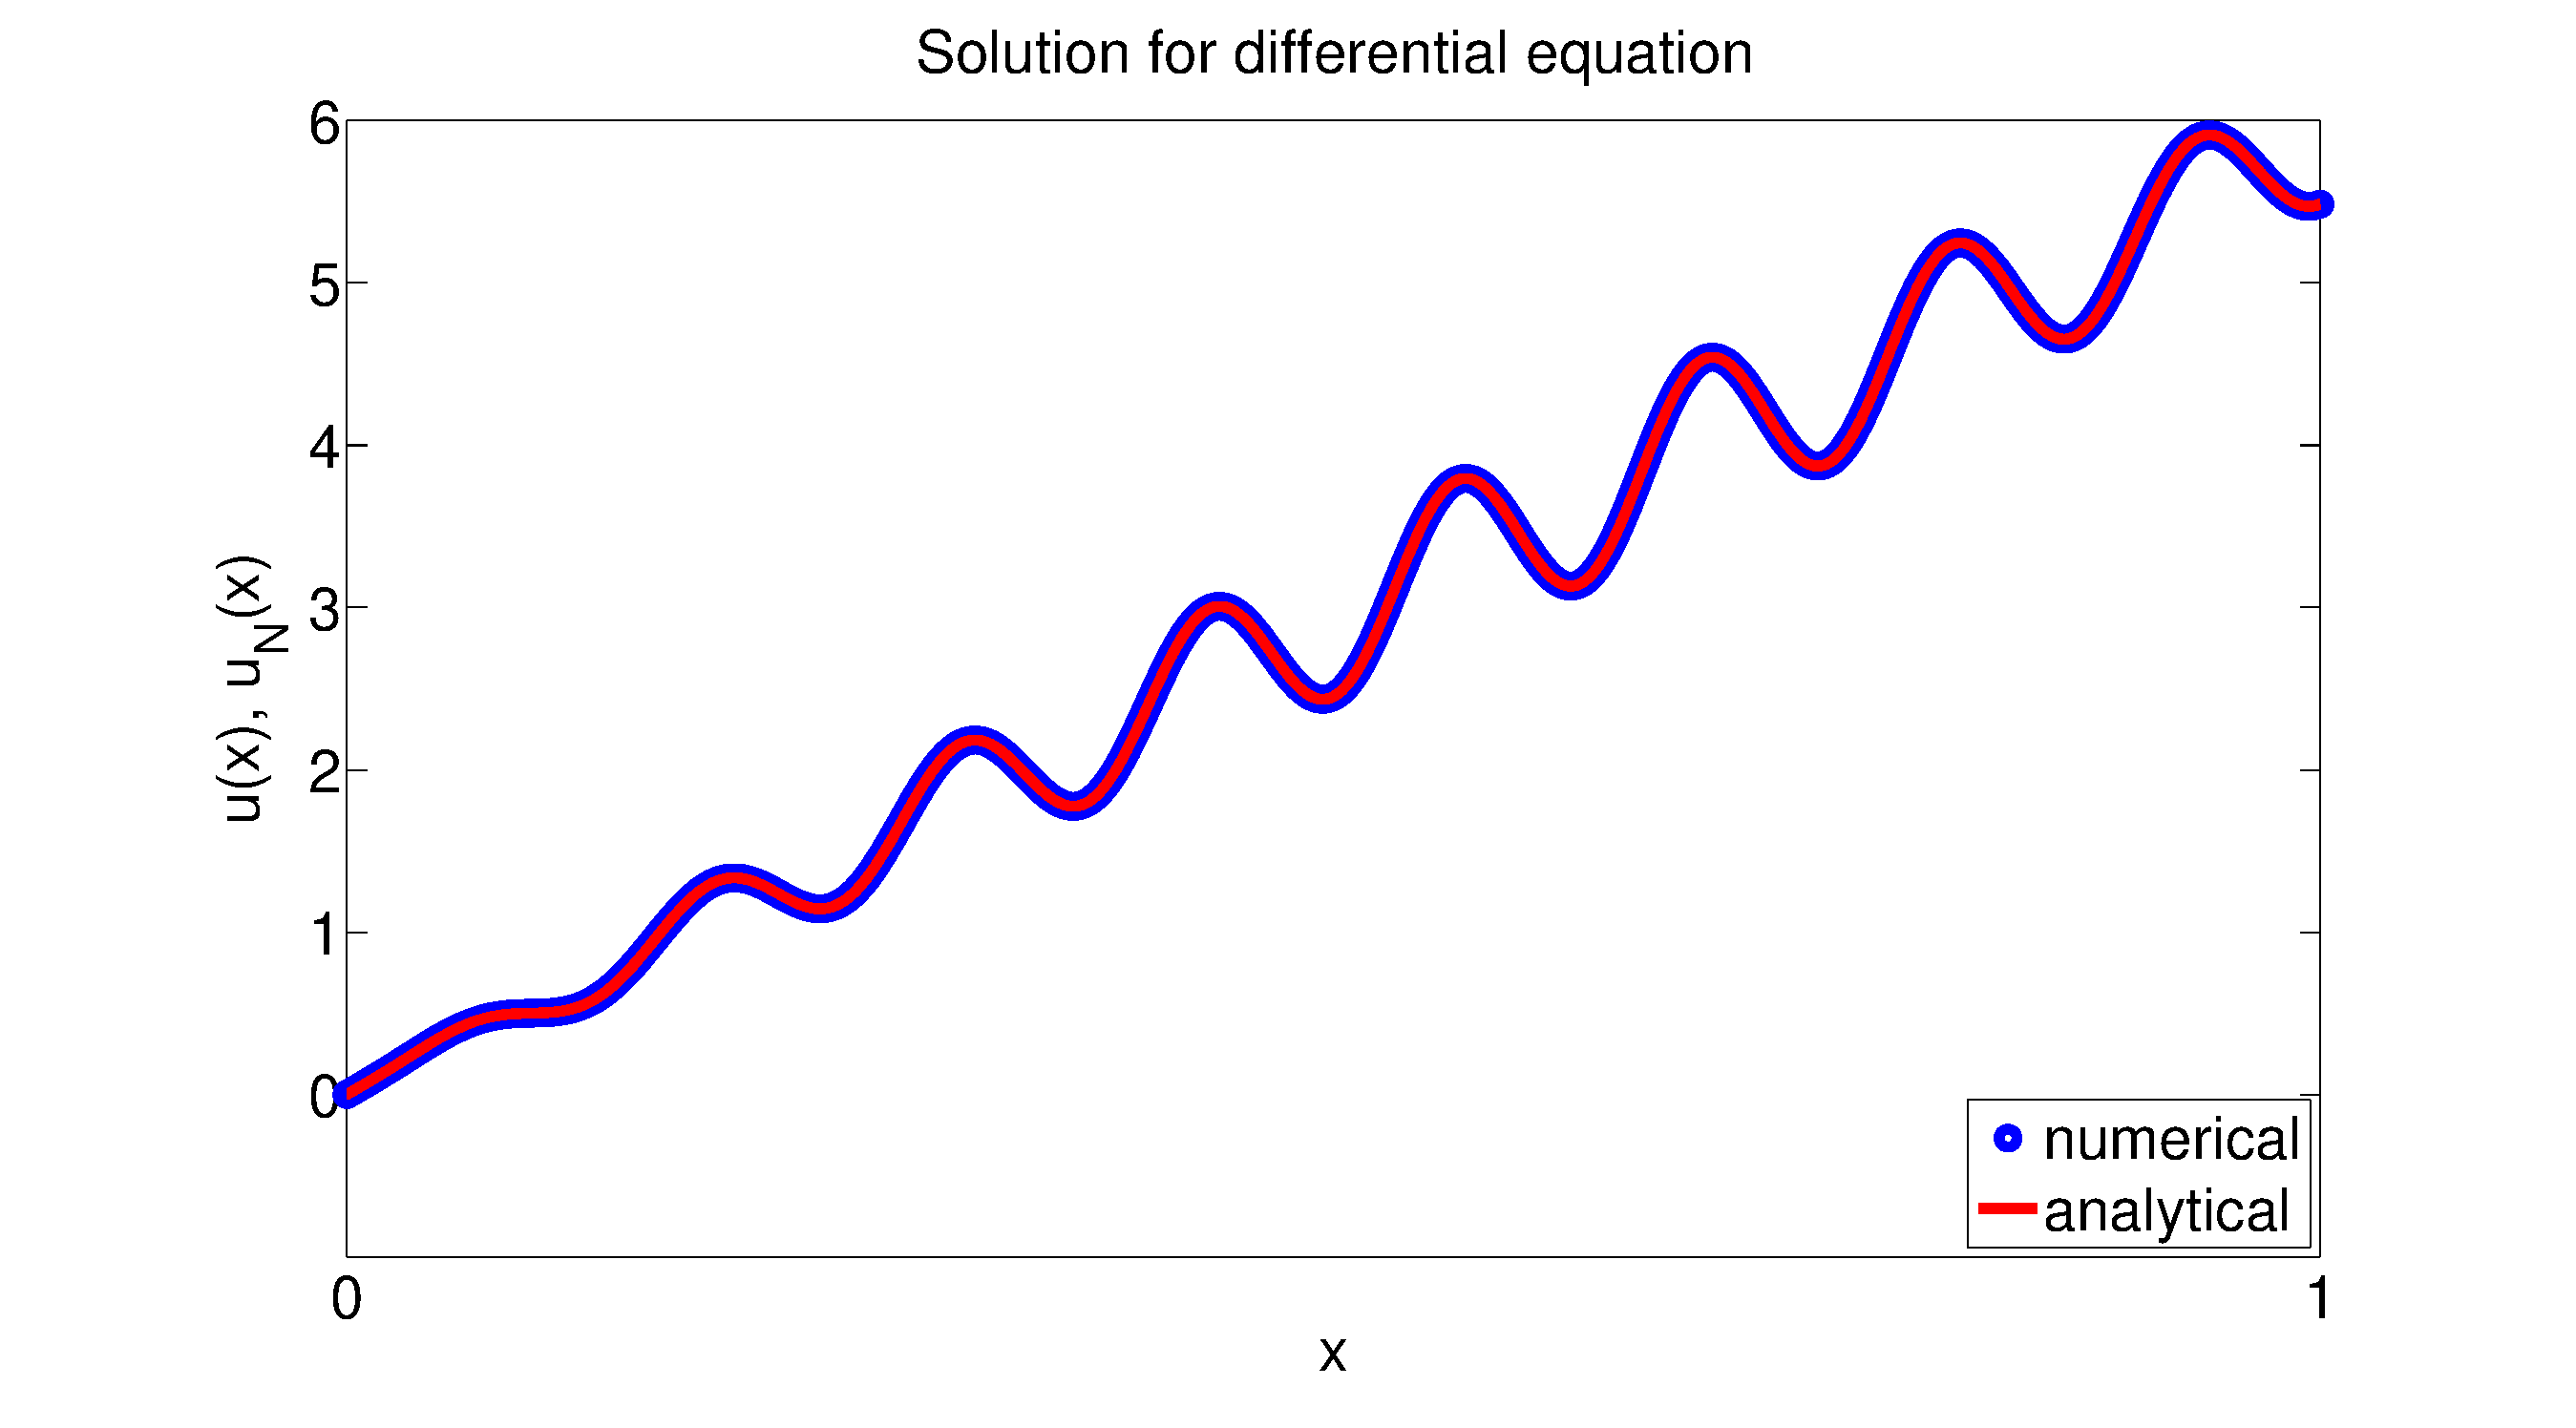
\includegraphics[width=\textwidth]{solution_P1.eps}
%                 \caption{linear element solution}
%                 \label{fig:k2}
%         \end{subfigure}%
%         %add desired spacing between images, e. g. ~, \quad, \qquad, \hfill etc.
%           %(or a blank line to force the subfigure onto a new line)
        
%         \begin{subfigure}[b]{\textwidth}
%                 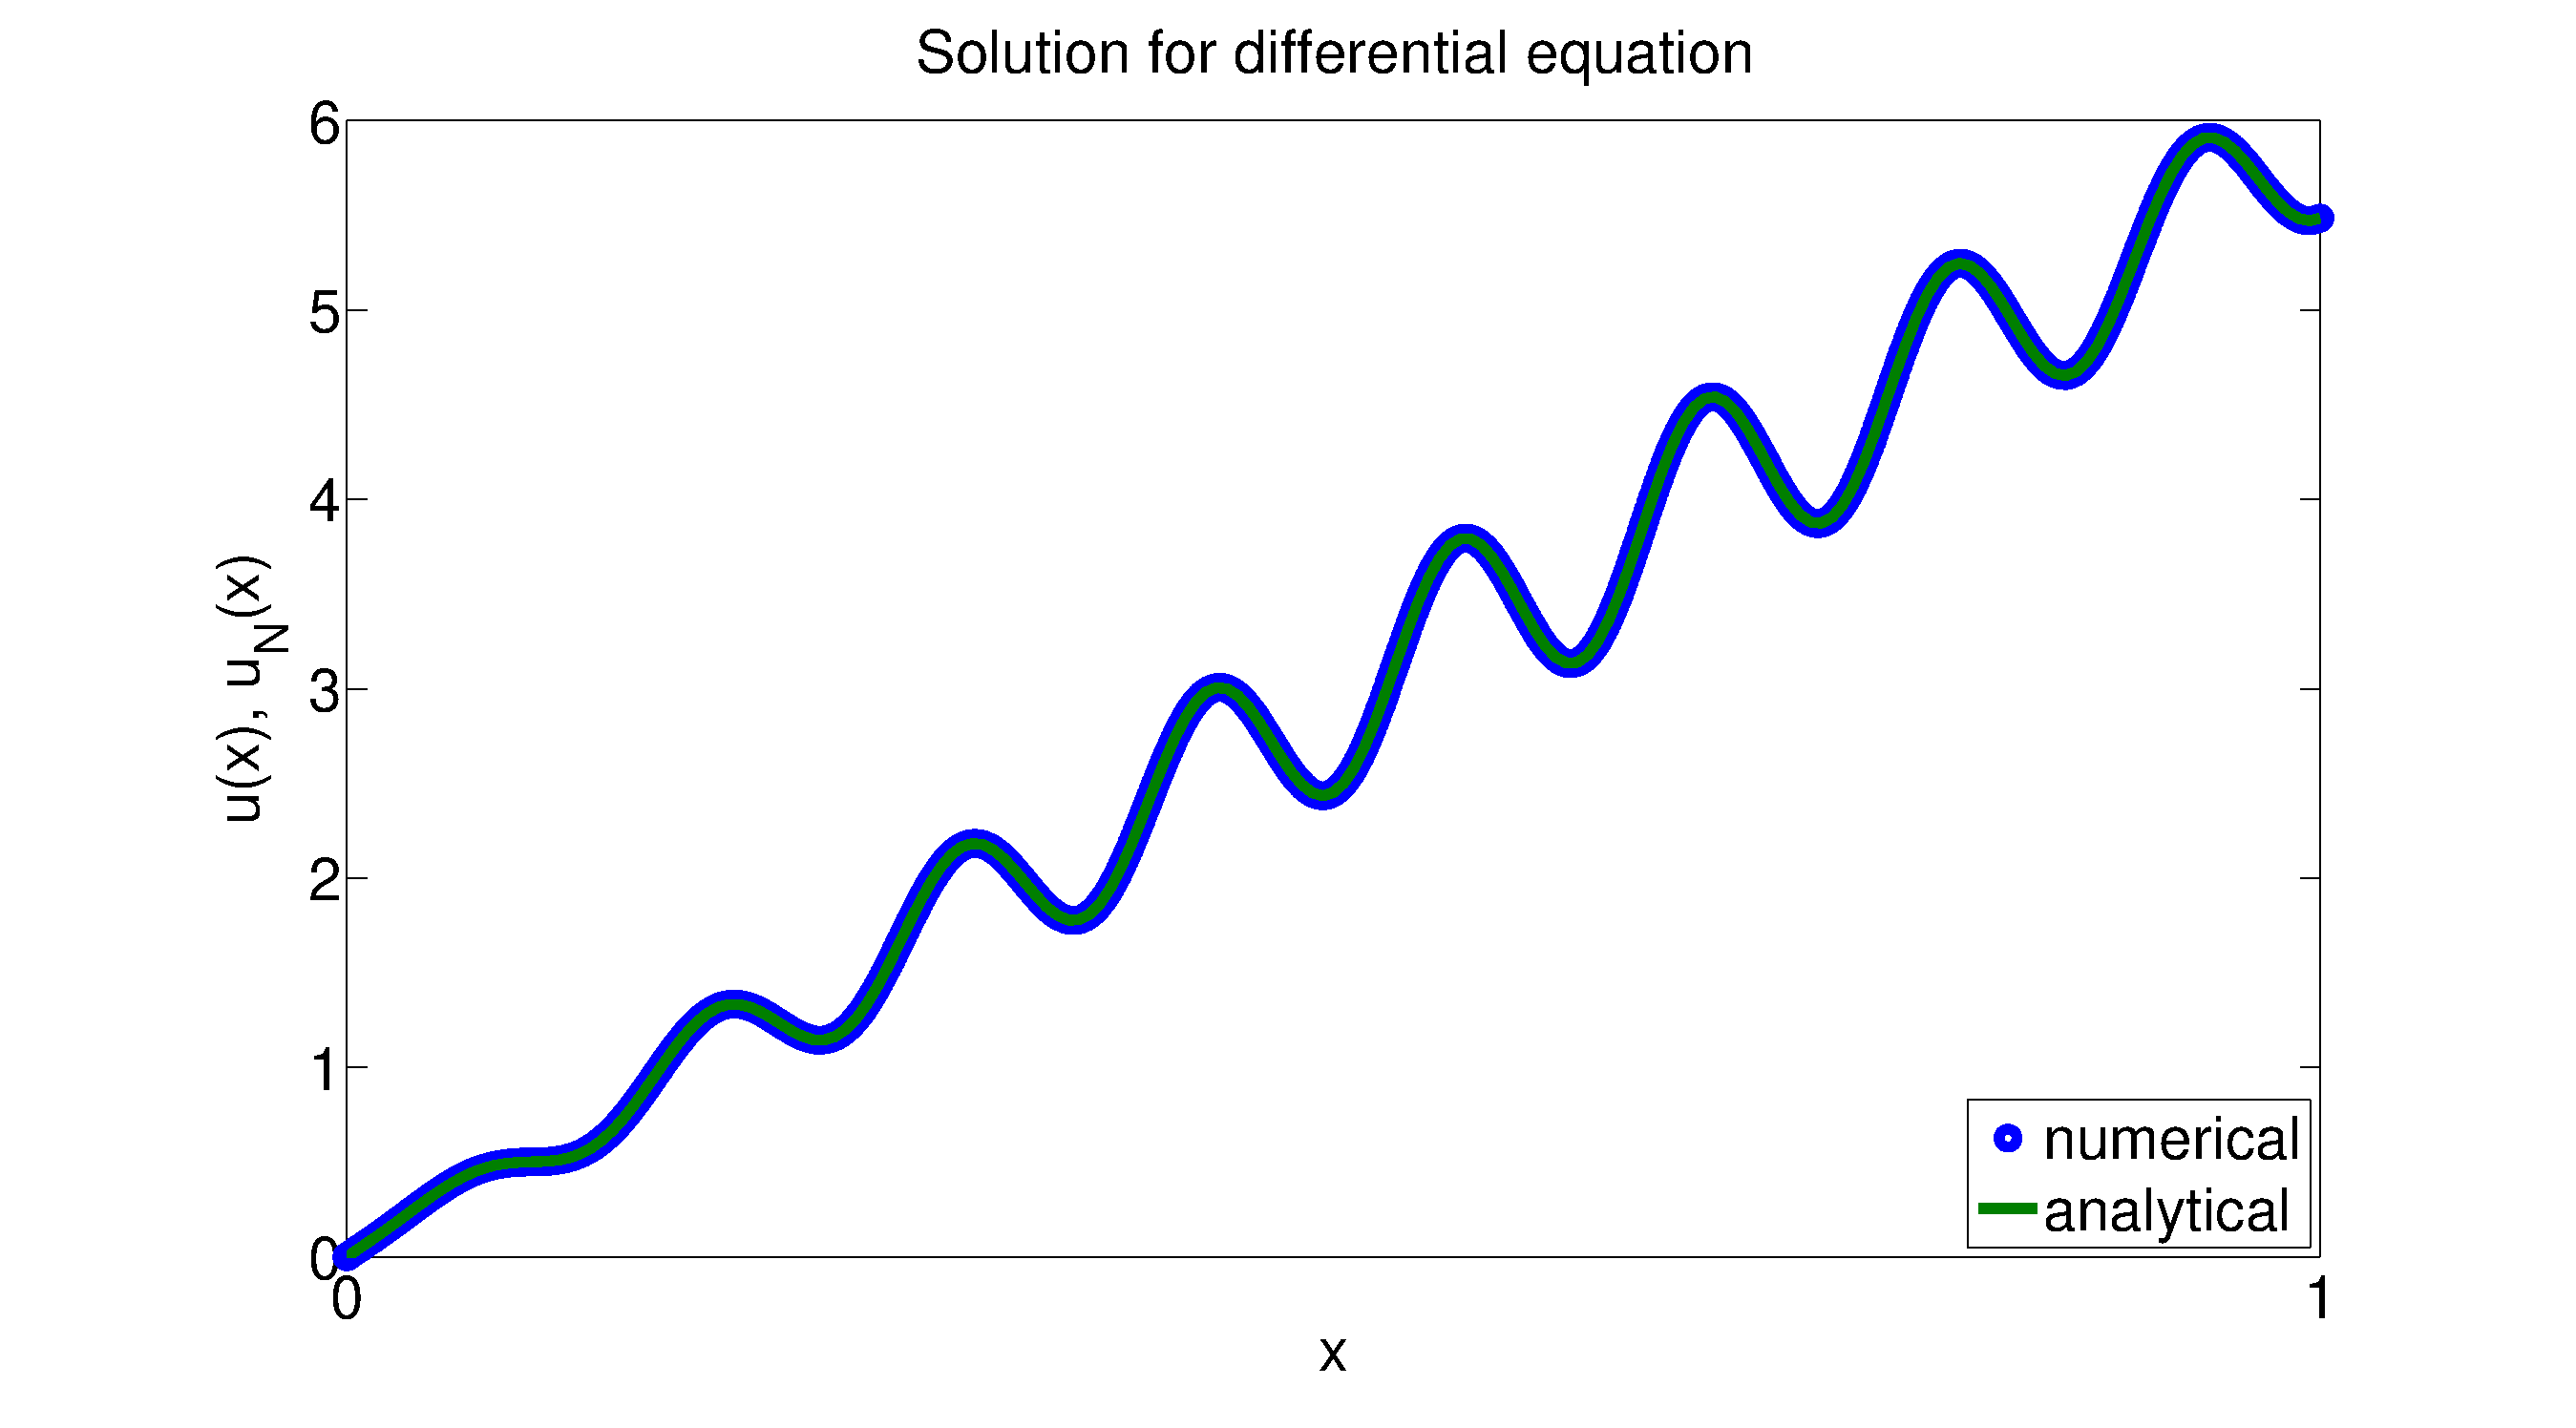
\includegraphics[width=\textwidth]{solution_P2.eps}
%                 \caption{quadratic element solution}
%                 \label{fig:k4}
%         \end{subfigure}
%         %add desired spacing between images, e. g. ~, \quad, \qquad, \hfill etc.
%           %(or a blank line to force the subfigure onto a new line)
        
%         \begin{subfigure}[b]{\textwidth}
%                 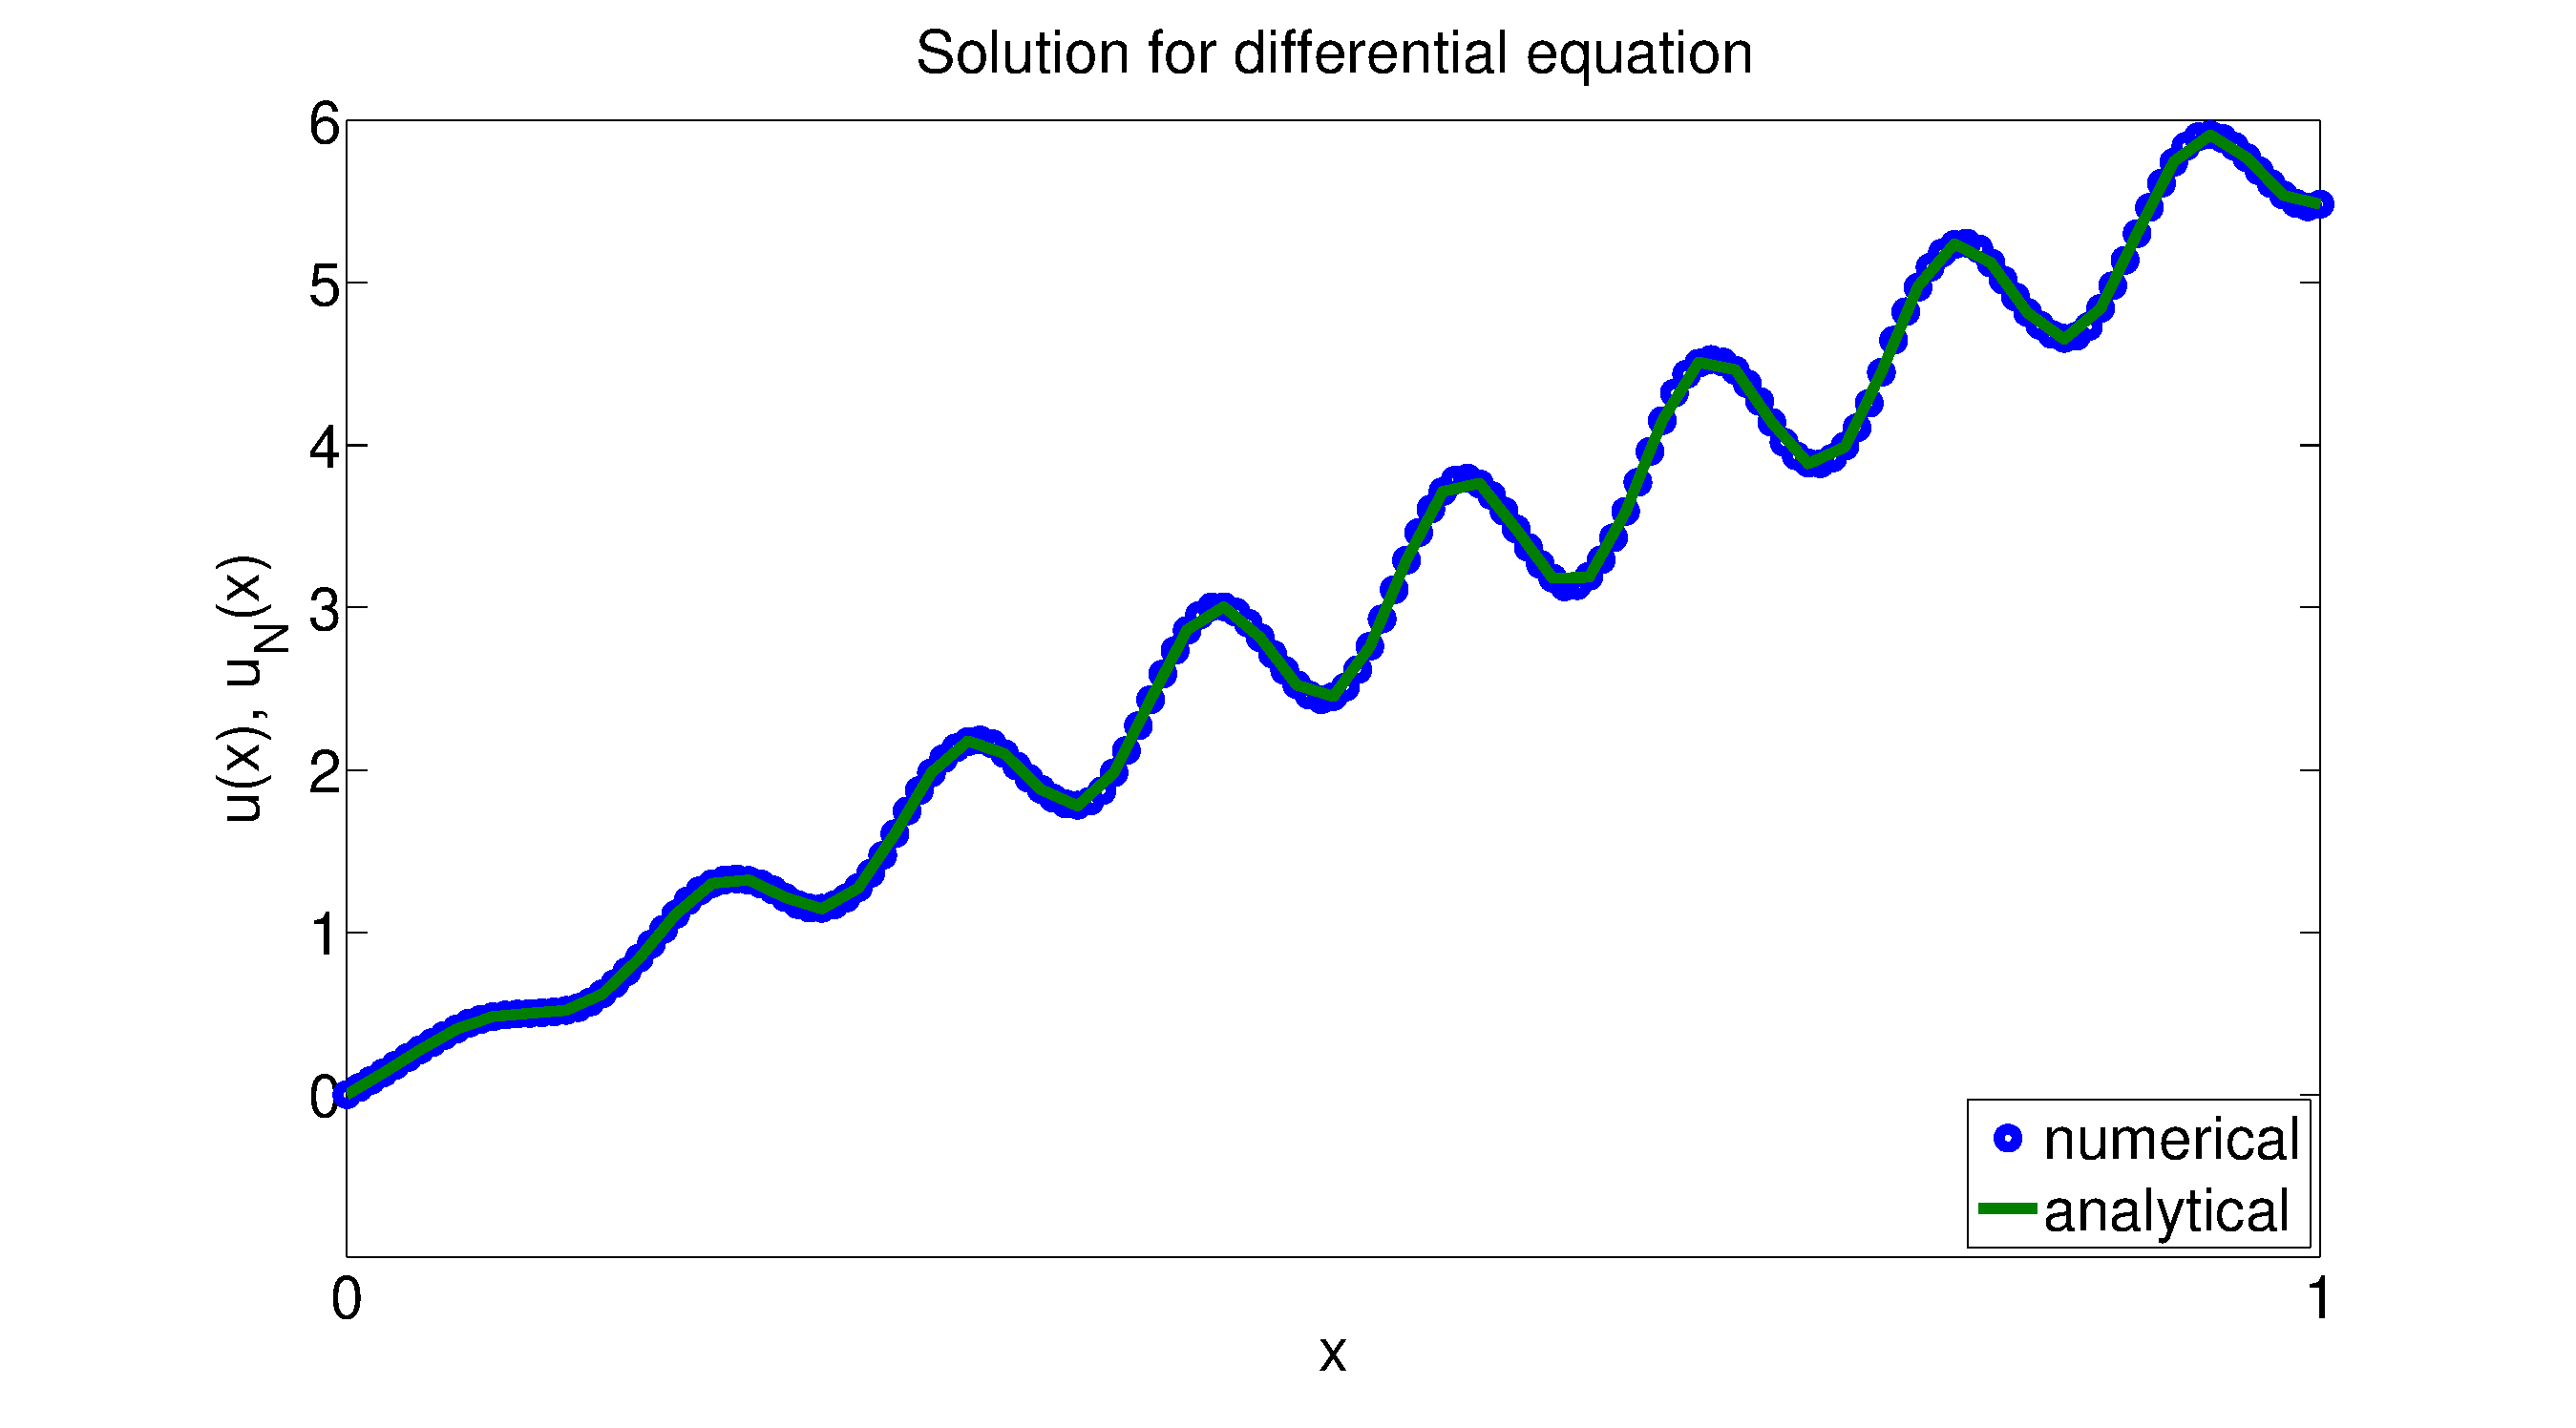
\includegraphics[width=\textwidth]{solution_P3.eps}
%                 \caption{cubic element solution}
%                 \label{fig:k8}
%         \end{subfigure}

%         \caption{Comparison of analytical solution and numerical solution at optimum number of element}\label{fig:solution}
% \end{figure}

\subsection{Relationship between the error and the element size}
Error estimate for FEM is:
\begin{eqnarray}
e^N \leq Ch^{\gamma = min (r-1, P)}
\end{eqnarray}
r is smoothness, and P is the polynomial order.

From the error plotting, we can observe the linear relation between $log(e^N)$ and $log(h)$, 

\begin{eqnarray}
\gamma = 0.98, P=1\nonumber\\
\gamma = 1.98, P=2\nonumber\\
\gamma = 2.93, P=3\nonumber\\
\end{eqnarray}

Overall, $\gamma$ is similar  to P. 

% \begin{figure}
%         \centering
%         \begin{subfigure}[b]{0.8\textwidth}
%                 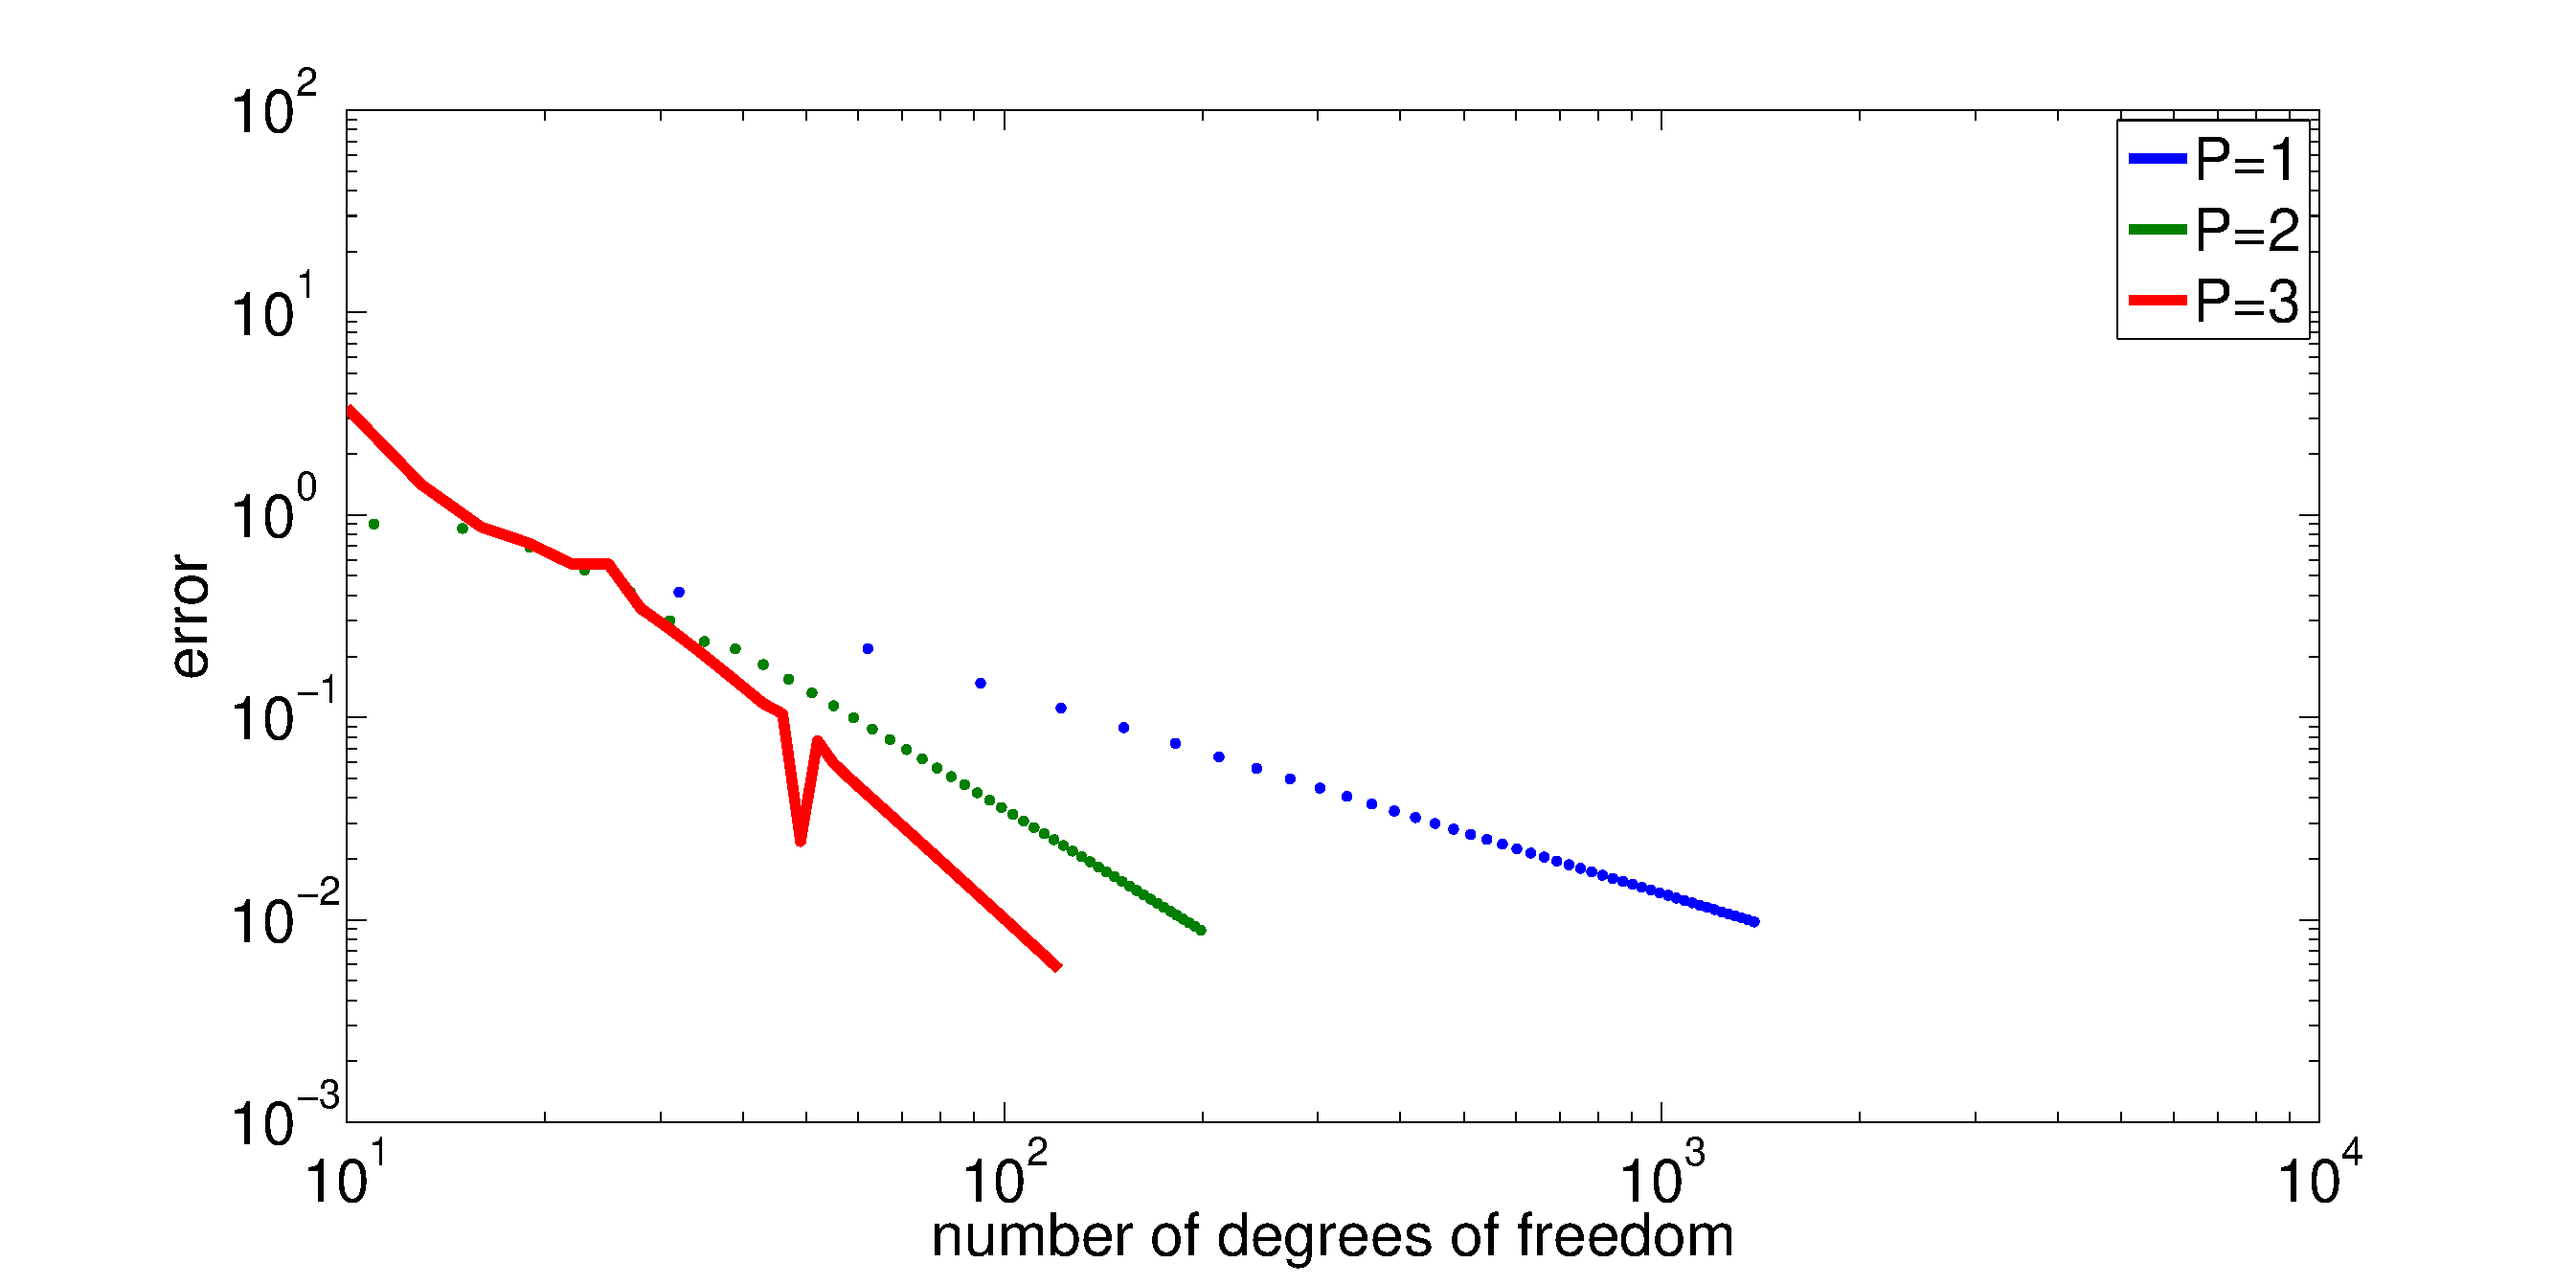
\includegraphics[width=\textwidth]{error_DOF.eps}
%                 \label{fig:e1}
%         \end{subfigure}

%         \caption{Evoluation of numerical error with number of elements}\label{fig:error}
% \end{figure}

% \begin{figure}
%         \centering
%         \begin{subfigure}[b]{0.8\textwidth}
%                 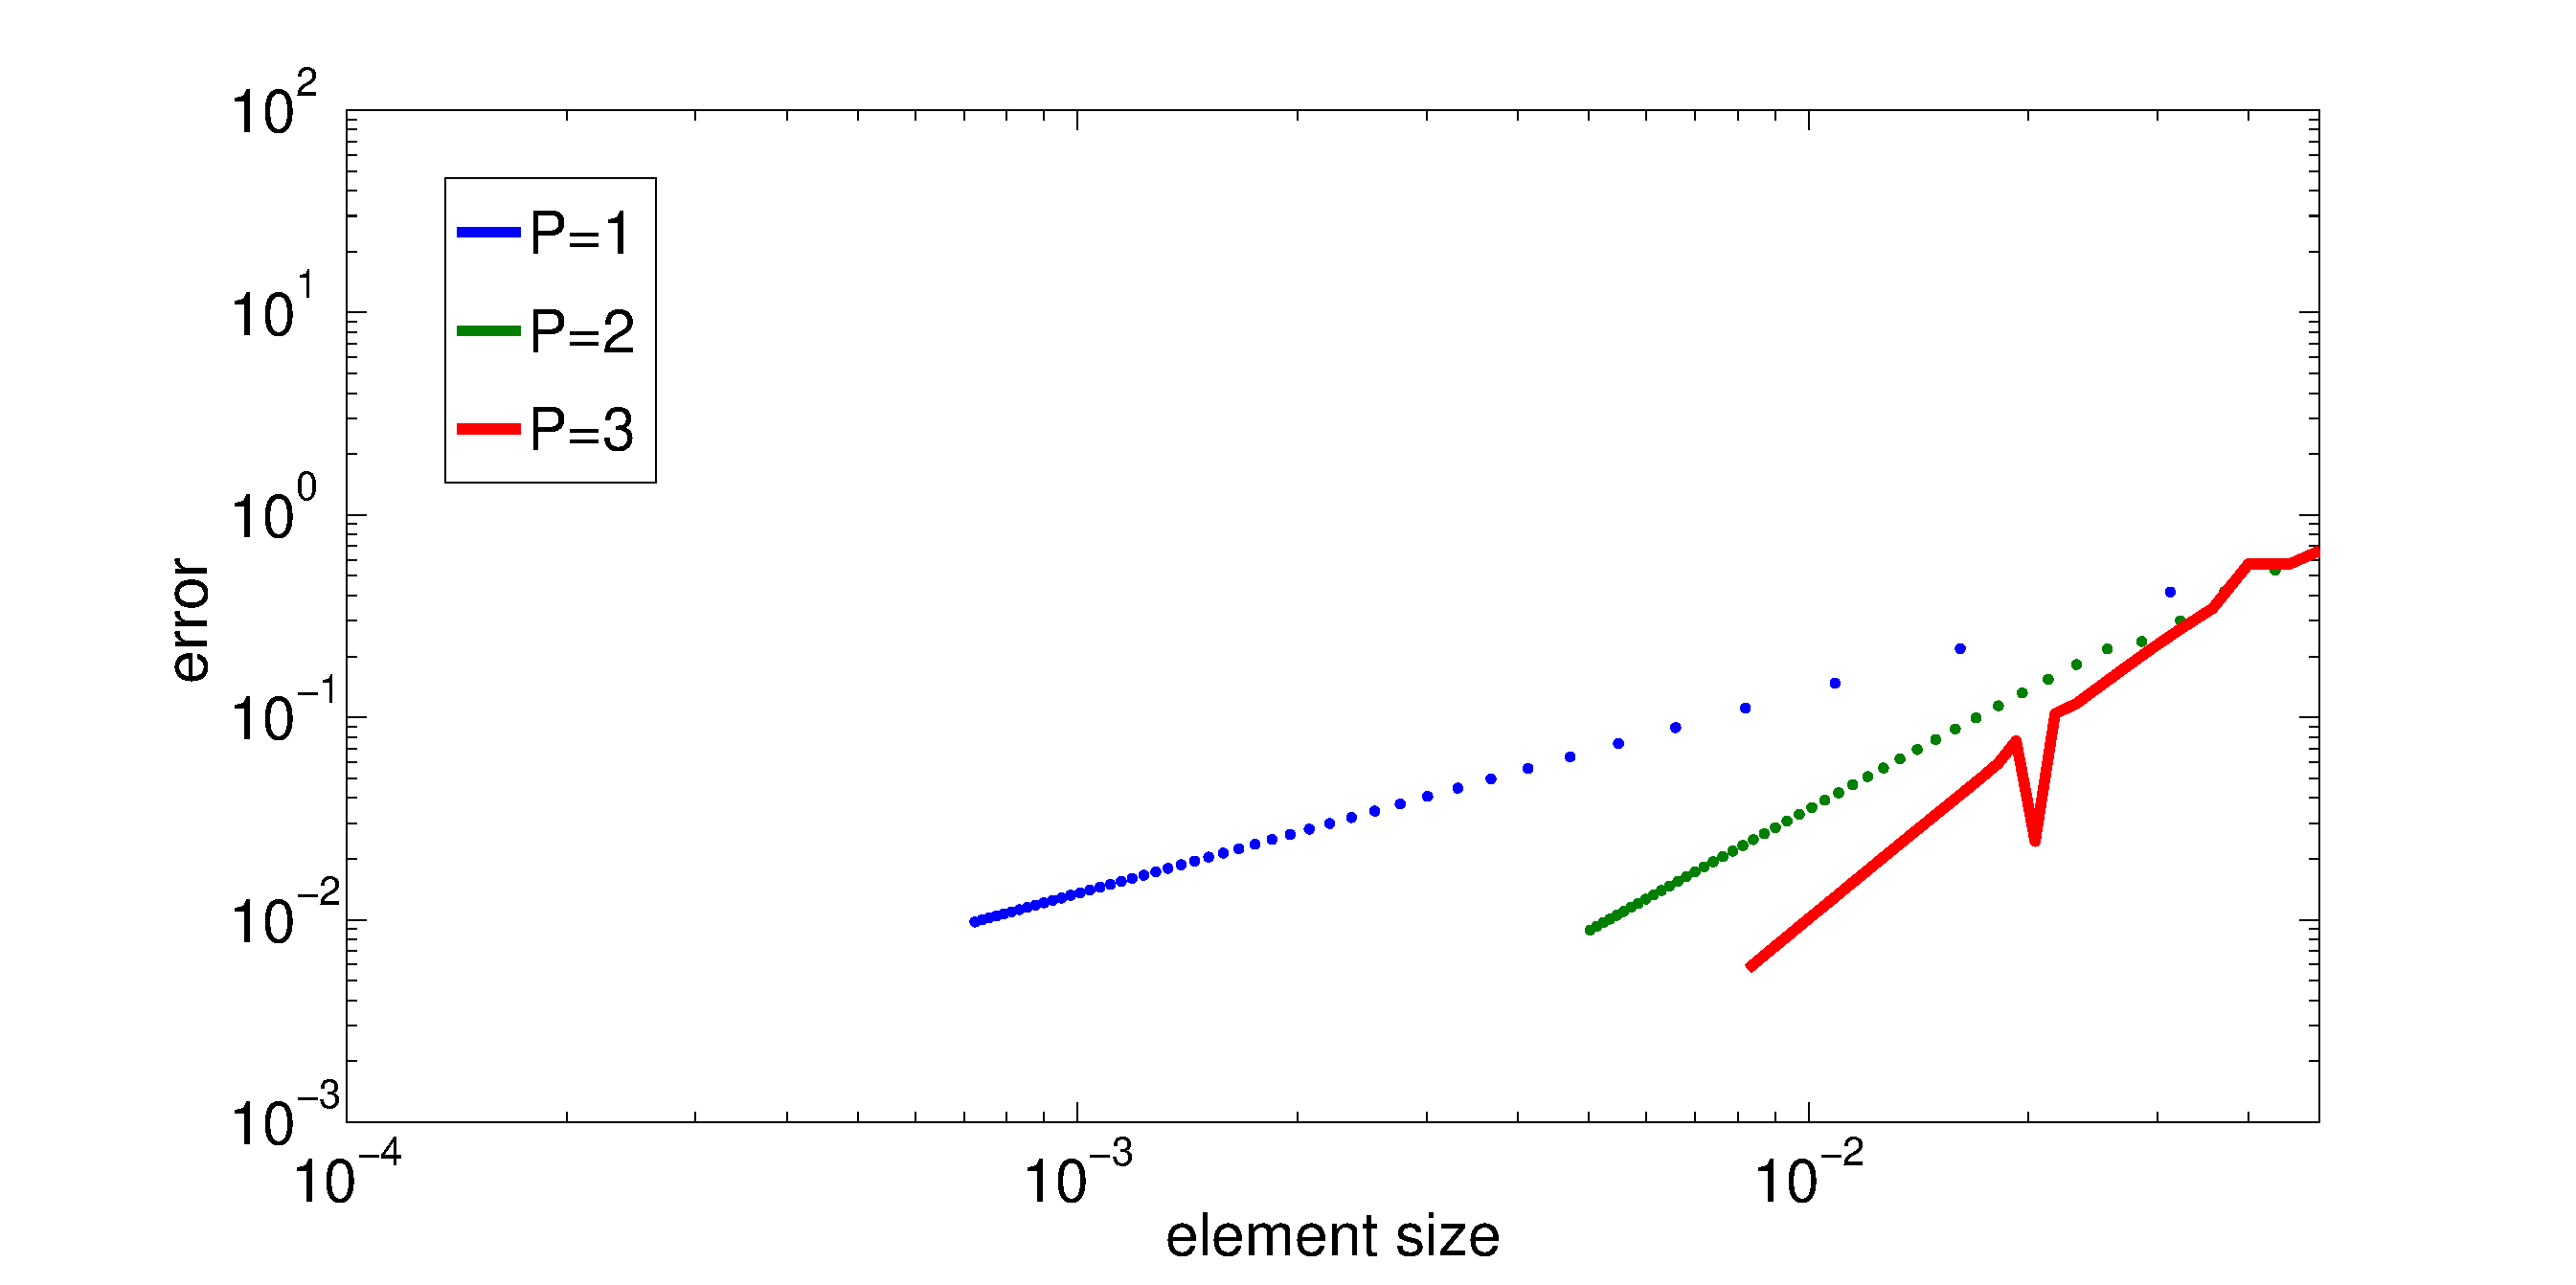
\includegraphics[width=\textwidth]{error_h.eps}
%                 \label{fig:e1}
%         \end{subfigure}

%         \caption{Evoluation of numerical error with number of elements}\label{fig:error}
% \end{figure}

\section{Conclusion}

This homework extends the previous one to higher order of element. Having higher order element shape functions can reduce the number of degree of freedom needed for solving the problem by better capturing the fluctuations in the solution. 

\end{document}